\exercise

Given the binary vectors A = 10111, B = 10010, C = 00010, D = 00000 and E =
01100, apply LSH to find the similar vectors according to Hamming distance,
given $k = 2$ and $L = 2$. \emph{(Hint: use projections $I_1 = \{0, 3\}$, $I_2 =
\{3, 4\}$)}

\solution

First, we construct the sketch of each vector:
%
\begin{figure}[H]
  \hfill
  \begin{minipage}{0.45\columnwidth}
  \centering
  \begin{tabular}{c|c|c}
    {\bf v} & $I_1(\text{\bf v})$ & $I_2(\text{\bf v})$ \\ \hline
    A & 11 & 11 \\
    B & 11 & 10 \\
    C & 01 & 10 \\
    D & 00 & 00 \\
    E & 00 & 00 \\
  \end{tabular}
  \end{minipage}
  \begin{minipage}{0.45\columnwidth}
  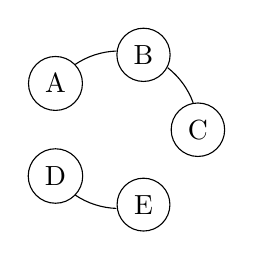
\begin{tikzpicture}
    \centering
    \def \radius {1cm}
    \def \margin {20}

    \node[draw, circle] at (0:\radius) {C};
    \draw[-, >=latex] ({0+\margin}:\radius)
      arc ({0+\margin}:{72-\margin}:\radius);
    \node[draw, circle] at (72:\radius) {B};
    \draw[-, >=latex] ({72+\margin}:\radius)
      arc ({72+\margin}:{144-\margin}:\radius);
    \node[draw, circle] at (144:\radius) {A};
    \node[draw, circle] at (216:\radius) {D};
    \draw[-, >=latex] ({216+\margin}:\radius)
      arc ({216+\margin}:{288-\margin}:\radius);
    \node[draw, circle] at (288:\radius) {E};

  \end{tikzpicture}
  \end{minipage}
  \hfill
\end{figure}
%
By the previous table, we can construct the similarity graph and conclude that:
%
\begin{itemize}
  \item A, B, C are similar;
  \item D, E are similar.
\end{itemize}

Alternatively, to speed up query time, we can construct an hash table for each
projection (each of size $2^{|I_i|}$) and use it as hash function, so to have:
%
\begin{table}[h]
  \centering
  \begin{tabular}{c|c|cc|c|c}
    \multicolumn{1}{c}{} &
    \multicolumn{1}{c}{$I_1$} &
    \multicolumn{1}{c}{} &
    \multicolumn{1}{c}{} &
    \multicolumn{1}{c}{$I_2$} & \\ \cline{2-2} \cline{5-5}
    00 & D, E & & 00 & D, E & \\ \cline{2-2} \cline{5-5}
    01 & C & & 01 & & \\ \cline{2-2} \cline{5-5}
    10 & & & 10 & B, C & \\ \cline{2-2} \cline{5-5}
    11 & A, B & & 11 & & \\ \cline{2-2} \cline{5-5}
  \end{tabular}
\end{table}

For example, given a new vector F = 11100, we compute the two projection,
$I_1(\text{F}) = 10$ and $I_2(\text{F}) = 00$, which point respectively to the
third and to the first cell of the two hash table, and find out that it is
similar to the vectors D and E. At this point we can compute explicitly the
Hamming distances:
%
\begin{align*}
  d(\text{F}, \text{D}) &= 3 \quad \text{\em (i.e., a false positive)},\\
  d(\text{F}, \text{E}) &= 1 \quad \text{\em (actually similar)}.
\end{align*}
